%% TeXtured 1.0.0 (2025-01-06)
%%%%%%%%%%%%%%%%%%%%%%%%%%%%%%%%%%%%%%%%%%%%%%%%%%%%%%%%%%%%%%%%%%%%%%%
%% NOTE: If you find any issues or have any suggestions, please open %%
%%       an Issue on GitHub: https://github.com/jdujava/TeXtured     %%
%%%%%%%%%%%%%%%%%%%%%%%%%%%%%%%%%%%%%%%%%%%%%%%%%%%%%%%%%%%%%%%%%%%%%%%

%% Enable built-in LaTeX support for PDF/A compliance (must be before `\documentclass`)
\DocumentMetadata{pdfversion=1.7, pdfstandard=A-2u}
%%% PDF/A compliance - glyph to Unicode mappings

%% NOTE: metadata are set up using the `hyperref` package in `preamble/general/hyperref.tex`

%% WARN: `pdfx` package is SUPERSEDED by built-in LaTeX support for PDF/A
%%       However, in case additional fonts are used, some glyphs may not be covered
%%       by default Unicode mappings, in which case they need to be mapped to Unicode
%%       code points manually (see below for GUIDE and examples).

%%% GUIDE: How to add missing unicode mappings for glyphs
%%
%% Consider following part of VeraPDF output for a non-compliant PDF:
%%   <rule specification="ISO 19005-2:2011" clause="6.2.11.7.2" testNumber="1" status="failed" passedChecks="0" failedChecks="1">
%%     <description>The Font dictionary of all fonts shall define the map of all used character codes to Unicode values,
%%                  either via a ToUnicode entry, or other mechanisms as defined in ISO 19005-2, 6.2.11.7.2.</description>
%%     <object>Glyph</object>
%%     <test>toUnicode != null</test>
%%     <check status="failed">
%%       <context>root/document[0]/pages[58](1323 0 obj PDPage)/contentStream[0](1324 0 obj PDContentStream)
%%                                          /operators[654]/usedGlyphs[0](RMTQUN+MSAM10 RMTQUN+MSAM10 57 0  0)</context>
%%       <errorMessage>The glyph can not be mapped to Unicode</errorMessage>
%%     </check>
%%   </rule>
%%
%% This means that some glyph on page 59 (indicated by a 0-based index `pages[58]`)
%% is missing a Unicode mapping. To fix this, we need to find the name of the glyph,
%% and provide a Unicode mapping for it. For further instructions how to proceed see
%% `preamble/pdfA-compliance/LaTeX-find-glyph-name/LaTeX-find-glyph-name.tex`.

\RequirePackage{iftex}
\ifluatex % only for luaLaTeX (sourced by default for pdfLaTeX)
    \RequirePackage{luatex85}
    %%% PDF/A compliance - glyph to Unicode mappings

%% NOTE: metadata are set up using the `hyperref` package in `preamble/general/hyperref.tex`

%% WARN: `pdfx` package is SUPERSEDED by built-in LaTeX support for PDF/A
%%       However, in case additional fonts are used, some glyphs may not be covered
%%       by default Unicode mappings, in which case they need to be mapped to Unicode
%%       code points manually (see below for GUIDE and examples).

%%% GUIDE: How to add missing unicode mappings for glyphs
%%
%% Consider following part of VeraPDF output for a non-compliant PDF:
%%   <rule specification="ISO 19005-2:2011" clause="6.2.11.7.2" testNumber="1" status="failed" passedChecks="0" failedChecks="1">
%%     <description>The Font dictionary of all fonts shall define the map of all used character codes to Unicode values,
%%                  either via a ToUnicode entry, or other mechanisms as defined in ISO 19005-2, 6.2.11.7.2.</description>
%%     <object>Glyph</object>
%%     <test>toUnicode != null</test>
%%     <check status="failed">
%%       <context>root/document[0]/pages[58](1323 0 obj PDPage)/contentStream[0](1324 0 obj PDContentStream)
%%                                          /operators[654]/usedGlyphs[0](RMTQUN+MSAM10 RMTQUN+MSAM10 57 0  0)</context>
%%       <errorMessage>The glyph can not be mapped to Unicode</errorMessage>
%%     </check>
%%   </rule>
%%
%% This means that some glyph on page 59 (indicated by a 0-based index `pages[58]`)
%% is missing a Unicode mapping. To fix this, we need to find the name of the glyph,
%% and provide a Unicode mapping for it. For further instructions how to proceed see
%% `preamble/pdfA-compliance/LaTeX-find-glyph-name/LaTeX-find-glyph-name.tex`.

\RequirePackage{iftex}
\ifluatex % only for luaLaTeX (sourced by default for pdfLaTeX)
    \RequirePackage{luatex85}
    %%% PDF/A compliance - glyph to Unicode mappings

%% NOTE: metadata are set up using the `hyperref` package in `preamble/general/hyperref.tex`

%% WARN: `pdfx` package is SUPERSEDED by built-in LaTeX support for PDF/A
%%       However, in case additional fonts are used, some glyphs may not be covered
%%       by default Unicode mappings, in which case they need to be mapped to Unicode
%%       code points manually (see below for GUIDE and examples).

%%% GUIDE: How to add missing unicode mappings for glyphs
%%
%% Consider following part of VeraPDF output for a non-compliant PDF:
%%   <rule specification="ISO 19005-2:2011" clause="6.2.11.7.2" testNumber="1" status="failed" passedChecks="0" failedChecks="1">
%%     <description>The Font dictionary of all fonts shall define the map of all used character codes to Unicode values,
%%                  either via a ToUnicode entry, or other mechanisms as defined in ISO 19005-2, 6.2.11.7.2.</description>
%%     <object>Glyph</object>
%%     <test>toUnicode != null</test>
%%     <check status="failed">
%%       <context>root/document[0]/pages[58](1323 0 obj PDPage)/contentStream[0](1324 0 obj PDContentStream)
%%                                          /operators[654]/usedGlyphs[0](RMTQUN+MSAM10 RMTQUN+MSAM10 57 0  0)</context>
%%       <errorMessage>The glyph can not be mapped to Unicode</errorMessage>
%%     </check>
%%   </rule>
%%
%% This means that some glyph on page 59 (indicated by a 0-based index `pages[58]`)
%% is missing a Unicode mapping. To fix this, we need to find the name of the glyph,
%% and provide a Unicode mapping for it. For further instructions how to proceed see
%% `preamble/pdfA-compliance/LaTeX-find-glyph-name/LaTeX-find-glyph-name.tex`.

\RequirePackage{iftex}
\ifluatex % only for luaLaTeX (sourced by default for pdfLaTeX)
    \RequirePackage{luatex85}
    \input{glyphtounicode.tex} % probably not loaded automatically for luatex
    \pdfgentounicode=1         % probably disabled by default for luatex
\fi

%% Enable in case some glyphs are missing from imported PDF figures
\pdfinclusioncopyfonts=1

%% Additional Unicode mappings for mathematical symbols (provided by `pdfx`)
%% https://gist.github.com/literalplus/045c4d090e2fe742157b4c903a984d24
\input{glyphtounicode-cmr.tex} % <- /usr/share/texmf-dist/tex/latex/pdfx/glyphtounicode-cmr.tex
% \input{glyphtounicode-ntx.tex} % <- /usr/share/texmf-dist/tex/latex/pdfx/glyphtounicode-ntx.tex


%%% Additional Unicode mappings for various extra glyphs

%% Glyphs: double brackets (of various sizes)
%% name of glyph found in /usr/share/texmf-dist/fonts/afm/public/stmaryrd/stmary5.afm
\pdfglyphtounicode{llbracket}{27E6} % https://codepoints.net/U+27E6
\pdfglyphtounicode{rrbracket}{27E7} % https://codepoints.net/U+27E7
\pdfglyphtounicode{largellbracket}{27E6 FE01} % variants according to size
\pdfglyphtounicode{largerrbracket}{27E7 FE01} % ... ... .. ....
\pdfglyphtounicode{Largellbracket}{27E6 FE02} % ... ... .. ....
\pdfglyphtounicode{Largerrbracket}{27E7 FE02} % ... ... .. ....
\pdfglyphtounicode{LARGEllbracket}{27E6 FE03} % ... ... .. ....
\pdfglyphtounicode{LARGErrbracket}{27E7 FE03} % ... ... .. ....
\pdfglyphtounicode{hugellbracket} {27E6 FE04} % ... ... .. ....
\pdfglyphtounicode{hugerrbracket} {27E7 FE04} % ... ... .. ....
\pdfglyphtounicode{Hugellbracket} {27E6 FE05} % ... ... .. ....
\pdfglyphtounicode{Hugerrbracket} {27E7 FE05} % ... ... .. ....
\pdfglyphtounicode{Hugellbrackettop}{23A5 23A1} % separate top, middle, bottom
\pdfglyphtounicode{Hugellbracketex} {23A5 23A2} % ... ... .. ....
\pdfglyphtounicode{Hugellbracketbot}{23A6 23A3} % ... ... .. ....
\pdfglyphtounicode{Hugerrbrackettop}{23A4 23A2} % ... ... .. ....
\pdfglyphtounicode{Hugerrbracketex} {23A5 23A2} % ... ... .. ....
\pdfglyphtounicode{Hugerrbracketbot}{23A6 23A2} % ... ... .. ....

%% Glyph: short minus
\pdfglyphtounicode{axisshort}{2212} % short minus -> minus https://codepoints.net/U+2212

%%% TODO: maybe use `\pdfstringdefDisableCommands` for something (in PDF metadata?)
 % probably not loaded automatically for luatex
    \pdfgentounicode=1         % probably disabled by default for luatex
\fi

%% Enable in case some glyphs are missing from imported PDF figures
\pdfinclusioncopyfonts=1

%% Additional Unicode mappings for mathematical symbols (provided by `pdfx`)
%% https://gist.github.com/literalplus/045c4d090e2fe742157b4c903a984d24
\input{glyphtounicode-cmr.tex} % <- /usr/share/texmf-dist/tex/latex/pdfx/glyphtounicode-cmr.tex
% \input{glyphtounicode-ntx.tex} % <- /usr/share/texmf-dist/tex/latex/pdfx/glyphtounicode-ntx.tex


%%% Additional Unicode mappings for various extra glyphs

%% Glyphs: double brackets (of various sizes)
%% name of glyph found in /usr/share/texmf-dist/fonts/afm/public/stmaryrd/stmary5.afm
\pdfglyphtounicode{llbracket}{27E6} % https://codepoints.net/U+27E6
\pdfglyphtounicode{rrbracket}{27E7} % https://codepoints.net/U+27E7
\pdfglyphtounicode{largellbracket}{27E6 FE01} % variants according to size
\pdfglyphtounicode{largerrbracket}{27E7 FE01} % ... ... .. ....
\pdfglyphtounicode{Largellbracket}{27E6 FE02} % ... ... .. ....
\pdfglyphtounicode{Largerrbracket}{27E7 FE02} % ... ... .. ....
\pdfglyphtounicode{LARGEllbracket}{27E6 FE03} % ... ... .. ....
\pdfglyphtounicode{LARGErrbracket}{27E7 FE03} % ... ... .. ....
\pdfglyphtounicode{hugellbracket} {27E6 FE04} % ... ... .. ....
\pdfglyphtounicode{hugerrbracket} {27E7 FE04} % ... ... .. ....
\pdfglyphtounicode{Hugellbracket} {27E6 FE05} % ... ... .. ....
\pdfglyphtounicode{Hugerrbracket} {27E7 FE05} % ... ... .. ....
\pdfglyphtounicode{Hugellbrackettop}{23A5 23A1} % separate top, middle, bottom
\pdfglyphtounicode{Hugellbracketex} {23A5 23A2} % ... ... .. ....
\pdfglyphtounicode{Hugellbracketbot}{23A6 23A3} % ... ... .. ....
\pdfglyphtounicode{Hugerrbrackettop}{23A4 23A2} % ... ... .. ....
\pdfglyphtounicode{Hugerrbracketex} {23A5 23A2} % ... ... .. ....
\pdfglyphtounicode{Hugerrbracketbot}{23A6 23A2} % ... ... .. ....

%% Glyph: short minus
\pdfglyphtounicode{axisshort}{2212} % short minus -> minus https://codepoints.net/U+2212

%%% TODO: maybe use `\pdfstringdefDisableCommands` for something (in PDF metadata?)
 % probably not loaded automatically for luatex
    \pdfgentounicode=1         % probably disabled by default for luatex
\fi

%% Enable in case some glyphs are missing from imported PDF figures
\pdfinclusioncopyfonts=1

%% Additional Unicode mappings for mathematical symbols (provided by `pdfx`)
%% https://gist.github.com/literalplus/045c4d090e2fe742157b4c903a984d24
\input{glyphtounicode-cmr.tex} % <- /usr/share/texmf-dist/tex/latex/pdfx/glyphtounicode-cmr.tex
% \input{glyphtounicode-ntx.tex} % <- /usr/share/texmf-dist/tex/latex/pdfx/glyphtounicode-ntx.tex


%%% Additional Unicode mappings for various extra glyphs

%% Glyphs: double brackets (of various sizes)
%% name of glyph found in /usr/share/texmf-dist/fonts/afm/public/stmaryrd/stmary5.afm
\pdfglyphtounicode{llbracket}{27E6} % https://codepoints.net/U+27E6
\pdfglyphtounicode{rrbracket}{27E7} % https://codepoints.net/U+27E7
\pdfglyphtounicode{largellbracket}{27E6 FE01} % variants according to size
\pdfglyphtounicode{largerrbracket}{27E7 FE01} % ... ... .. ....
\pdfglyphtounicode{Largellbracket}{27E6 FE02} % ... ... .. ....
\pdfglyphtounicode{Largerrbracket}{27E7 FE02} % ... ... .. ....
\pdfglyphtounicode{LARGEllbracket}{27E6 FE03} % ... ... .. ....
\pdfglyphtounicode{LARGErrbracket}{27E7 FE03} % ... ... .. ....
\pdfglyphtounicode{hugellbracket} {27E6 FE04} % ... ... .. ....
\pdfglyphtounicode{hugerrbracket} {27E7 FE04} % ... ... .. ....
\pdfglyphtounicode{Hugellbracket} {27E6 FE05} % ... ... .. ....
\pdfglyphtounicode{Hugerrbracket} {27E7 FE05} % ... ... .. ....
\pdfglyphtounicode{Hugellbrackettop}{23A5 23A1} % separate top, middle, bottom
\pdfglyphtounicode{Hugellbracketex} {23A5 23A2} % ... ... .. ....
\pdfglyphtounicode{Hugellbracketbot}{23A6 23A3} % ... ... .. ....
\pdfglyphtounicode{Hugerrbrackettop}{23A4 23A2} % ... ... .. ....
\pdfglyphtounicode{Hugerrbracketex} {23A5 23A2} % ... ... .. ....
\pdfglyphtounicode{Hugerrbracketbot}{23A6 23A2} % ... ... .. ....

%% Glyph: short minus
\pdfglyphtounicode{axisshort}{2212} % short minus -> minus https://codepoints.net/U+2212

%%% TODO: maybe use `\pdfstringdefDisableCommands` for something (in PDF metadata?)


%% NOTE: Choose the desirable page layout version (electronic vs print)
\documentclass[12pt,a4paper]{report}                      % single-side (electronic)
% \documentclass[12pt,a4paper,openright,twoside]{report}  % two-sided (for printing)

\newif\ifWIP
\newif\ifCENSOR
%% NOTE: Comment out the following lines for the final version
\WIPtrue % THIS IS A WORK-IN-PROGRESS VERSION
\CENSORtrue % THIS IS A CENSORED VERSION

\newif\ifFANCY
\FANCYtrue % enable some of the more fancy stylistic choices

%% Preamble - data, packages, macros, and more
% Plantilla creada por Francisco Javier Vázquez Tavares
% Esta platilla se creo para facilitar la creación de documentos para tareas.

\documentclass{tareaClass}
%\selectlanguage{spanish} 
%\usepackage[spanish,onelanguage]{algorithm2e} %for psuedo code
\usepackage{listings}

\DeclareSIUnit\atm{atm}
\DeclareSIUnit\torr{torr}
\DeclareSIUnit\celcius{C}

\newcommand{\hata}{\hat{a}}
\newcommand{\hatad}{\hat{a}^\dagger}
\newcommand{\QDi}{\hat{X}_1}
\newcommand{\QDj}{\hat{X}_2}
%\usepackage[mathscr]{euscript}

\usepackage{mathrsfs}

\usepackage{tabularx}
\usepackage{booktabs}
\usepackage{multirow}

\materia{Smart Materials}
\profe{Dr. Mallar Ray}
\title{Problem set \#1: Piezoelectric Materials}
%\title{ Equilibrium in ideal gas reactions}
%\title{ Final Review practice problems }

\integrantes{Francisco Javier Vázquez Tavares}
\matriculas{A00827546}
%\date{18 de Agosto 2023}

\begin{document}
\lhead{Problem set 1: Piezoelectric Materials}\rhead{ September 5, 2025}

\maketitle

\subfile{docs/hwk1.tex}

%\printbibliography[heading=bibintoc,title={References}]

%\newpage

%\section{Appendix}
%\subfile{docs/hwk3.A.tex}
%\printbibliography[type=article,title={Artículos}]
%\printbibliography[type=book,title={Libros}]
%\printbibliography[type=online,title={Web}]
%\maketitle


\end{document}


%% Only uncommented files are included (faster compilation)
%% NOTE: If no files are uncommented, all files are included
\includeonlysmart{
    % frontmatter/title,
    % frontmatter/declaration,
    % frontmatter/dedication,
    % frontmatter/information,
    % chapters/Introduction,
    % chapters/QuickSummary,
    % chapters/Notation,
    % chapters/Design,
    % chapters/Usage,
    % chapters/Features,
    % chapters/Tips,
    % chapters/Summary,
    % chapters/Appendix,
}

\begin{document}

\frontmatter
\currentpdfbookmark{Title Page}{titlepage} % add PDF outline entry
\thispagestyle{empty} % no number on the title page
\begin{center}
    \begin{adjustbox}{center,trim=0 0.2cm 4cm 0.2cm}
        
\includegraphics[width=1.5\textwidth]{MFF-logo.pdf}
    \end{adjustbox}

    \Large

    \vspace{-2em}
    \vfill

    {\ifFANCY\sffamily\Huge\else\bfseries\LARGE\fi
        \MakeUppercase{\ThesisType} THESIS}

    \vfill

    {\Huge
        \ThesisAuthor}

    \vspace{1em}

    %% if `\ThesisTitleFront` is not defined, use `\ThesisTitle`
    \ProvideExpandableDocumentCommand{\ThesisTitleFront}{}{\ThesisTitle}
    % {\Huge \bfseries \ThesisTitleFront \par}
    {\fontsize{30pt}{36pt}\selectfont \sffamily\bfseries
        \ThesisTitleFront \par}

    \vfill

    \Department

    \vspace{1.1em}

    \begin{center}
        \large
        \renewcommand{\arraystretch}{1.2}
        \begin{tabular}{>{\sffamily\color{Gray40}}r @{\hspace{1.0em}} l}
            Supervisor of the Thesis    & \Supervisor     \\
            \ifdef{\CoSupervisor}{%
            Co-Supervisor of the Thesis & \CoSupervisor   \\
            }{}
            \ifdef{\StudyProgramme}{% TODO: programme vs program?
            Study Programme             & \StudyProgramme \\
            }{}
        \end{tabular}
    \end{center}

    \vspace{2em}

    \ifFANCY\sffamily\fi
    Prague \YearSubmitted \\
    \ifdef{\YearRevision}{%
        \emph{Revised version \YearRevision} \par
    }{}
    \ifWIP
        \small\ttfamily \textcolor{red}{(Draft - \today)} \par
    \fi
\end{center}

\newpage

% %%% A page with a solemn declaration

\cleardoublepage
\markboth{Declaration of Authorship}{Declaration of Authorship}
\vspace*{\fill}

\subsection*{Declaration of Authorship}

I declare that I carried out this \ThesisType{} thesis on my own, and only with the cited sources, literature and other professional sources.
I understand that my work relates to the rights and obligations under the Act No.~121/2000 Sb., the~Copyright Act, as amended, in particular the fact that the Charles University has the right to conclude a license agreement on the use of this work as a school work pursuant to Section 60 subsection 1 of the Copyright Act.

\vspace{7ex}

\begin{center}
    \renewcommand{\arraystretch}{1.3}
    \begin{tabular}{W{c}{0.32\linewidth} p{2em} W{c}{0.42\linewidth}}
        \arrayrulecolor{Gray70} \cmidrule{1-1} \cmidrule{3-3} % gray placeholder lines
        \emph{Place \& Date} && \emph{\ThesisAuthor} \\
    \end{tabular}
\end{center}

\vspace{5em}
\newpage

% \cleardoublepage
\markboth{Dedication}{Dedication}

{ \slshape
    Write dedication here.
}

\vfill

% %%% Mandatory information page of the thesis

%% NOTE: MFF guidelines can be found at
%% https://www.mff.cuni.cz/cs/vnitrni-zalezitosti/predpisy/opatreni-dekana/opatreni-dekana-c-27-2023
%%     -> no special formatting is required, so it should be fine to customize it

\cleardoublepage

% \chapternotnumbered{Information \& Abstract}
\phantomsection
\addcontentsline{toc}{chapter}{Information \& Abstract}
\markboth{Information \& Abstract}{Information \& Abstract}

\subsection*{Information}

\begin{tblr}{
        colspec = {r X},
        column{1} = {font=\small\sffamily\color{Gray40}},
        column{2} = {font=\small},
    }
    Title       & \ThesisTitle                             \\
    Author      & \ThesisAuthor                            \\
    \DeptType{} & \Department                              \\
    Supervisor  & \Supervisor{} --- \SupervisorsDepartment \\
    % Abstract    & \Abstract                                \\
    Keywords    & \Keywords                                \\
\end{tblr}

\subsection*{Abstract}

\Abstract


\contents

\chapternotnumbered{Introduction} \label{ch:Introduction}

Already when I started writing my bachelor thesis \autocite{Dujava2022}, I tweaked a lot the original \LaTeX{} template (which itself was slightly updated since then \autocite{MaresTemplate}) provided for students at MFF CUNI --- Faculty of Mathematics and Physics, Charles University in Prague.

Some design choices originated already during this stage, particularly the significant use of theorem-like and remark-like environments with highly interlinked structure of the text.

I picked up right where I left off when I started writing my master thesis \autocite{TODO}, and I have been refining the template ever since.
Improved understanding of the coding backbone behind \LaTeX{} and its package ecosystem enabled me to customize it even further to my liking, and add even more \enquote{bells and whistles}.

\begin{remark}[Template Purpose]
    While primarily targeting theses, \TeXtured{} can be used for other document types as well.
\end{remark}

To make it user-friendly, I have restructured the preamble into several files, each of which is responsible for a specific aspect of the document.
This way, the user can (and is encouraged to) easily find the relevant part of the code and modify it.

Numerous comments and explanations are provided throughout the code to further aid the user in understanding the template without always having to consult the documentation of packages (which is recommended for more advanced changes).

\begin{remark}[How to Setup]
    To set up \TeXtured{} template for your document, you can use the \texttt{Overleaf} template or clone the repository on \textsf{GitHub} \autocite{TeXtured}.
    Then, you can start modifying the files to suit your needs.

    Also make sure to check the \texttt{README.md} file for more detailed instructions, particularly on various software dependencies.
    If you encounter any issues, please see \href{https://github.com/jdujava/TeXtured/issues/2}{\texttt{jdujava/TeXtured \#2}} and \href{https://github.com/jdujava/TeXtured/issues/5}{\texttt{jdujava/TeXtured \#5}}.
\end{remark}

% \setcounter{chapter}{16} % "Q" (17th letter, but latex first increments -> 17-1=16)
% \chapter{Quick Summary}
\chapternotnumbered{Quick Summary} \label{ch:Quick Summary}

\vspace{2ex} % extra vertical space, since letter Q has a long tail


In \textbf{\Cref*{ch:notation}} we exhibit an example of a \emph{front matter} chapter.
%% TODO: maybe use \nameref{}, and more fluid description of chapters

\makebox{In \textbf{\Cref*{ch:Design}}} we present design \emph{Principles} to which \TeXtured{} adheres.
%% NOTE: `\makebox` is used to fix the width of "In Chapter X" part

\makebox{In \textbf{\Cref*{ch:Usage}}} we explain the file structure and the basics of using the template.

\makebox{In \textbf{\Cref*{ch:Features}}} we describe various implemented features, design choices, and \LaTeX{} packages helping with the task of realizing goals sketched in \Cref*{ch:Design}.

\makebox{In \textbf{\Cref*{ch:Tips}}} we give tips and tricks on how to fully utilize and even extend capabilities of \TeXtured{}.

In \textbf{\Cref*{appendix:example}} we show an example of an Appendix chapter.

\begin{Note}[WIP Disclaimer]
    Both \Cref{ch:Features} and \Cref{ch:Tips} are as of now Work-in-Progress.
    There is a lot of stuff yet to be exhibited and explained.
    All the colored \textsf{TODO}-like environments are to be resolved in the final version of this document.
\end{Note}

\setcounter{chapter}{13} % "N" (14th letter, but latex first increments -> 14-1=13)
\chapter{Notation \& Conventions} \label{ch:notation}
% NOTE: since we are in the "frontmatter" part, we need to manually set headers
%       we didn't use `\chapternotnumbered`, because we want its letter in TOC,
%       and the numbering of environments to be of the form "N.1"
\markboth{Notation \& Conventions}{Notation \& Conventions}

\vspace{2ex}

\begin{remark}
    This chapter is numbered (or perhaps more precisely \enquote{lettered}).
    This means that is appears in Table of Contents with its letter \enquote{\textbf{\textsf{N}}}, which also prefixes all numbering of environments in this chapter.

    On the other hand, \Nref{ch:Introduction} and \Nref{ch:Quick Summary} are unnumbered (or \enquote{unlettered}) in this sense.
\end{remark}

\begin{example}[Usage of Mathematical Fonts]
    To make the text more readable and beautiful, we can use different types of mathematical fonts for different types of objects (striving to be at least somewhat consistent):
    \begin{itemize}
        \item \(\bm{Bold}\) often for tensorial object (abstract index).
        \item \(\mathsf{Sans}\) for groups, certain spaces, or some operations/maps.
        \item \(\mathfrak{Fraktur}\) for algebras (and densities).
        \item \(\mathcal{C}a\ell\ell igraphic\) (available are only capital letters, and \(\ell\))
        \item \(\mathpzc{Calligraphic}\) (alternative font containing also lowercase letters)
        \item \(\mathbb{D}\)ouble-\(\mathbb{S}\)truck for fields like \(\R\), spaces like \(\Sphere^{n}\) and \(\CP^{n}\).
        \item \(\mathtt{Typewriter}\) for code functions, or other special objects. \qedhere
    \end{itemize}
\end{example}

\begin{example}
    You can use \(\mspace{1mu}\argument\mspace{1mu}\) as an argument placeholder.
\end{example}


\mainmatter
\chapter{Design Principles} \label{ch:Design}

It is not like I stated the \emph{Principles} at the beginning and then tried to follow them.
They emerged more naturally.
So the causal structure is more like
\[
    \raisebox{-0.15ex}{\parbox[c]{6em}{\centering made some design choices}}
    \mspace{12mu} \text{and} \mspace{10mu}
    \parbox[c]{7em}{\centering implemented certain features}
    \quad\longleadsto{}\quad
    \parbox[c]{10em}{\centering recognized\\\textcolor{gray}{at first subconscious} overarching principles}~.
\]
Anyway, here they are.
\begin{definition}[Design Principles] \label{def:Design Principles}
    The main design \emph{Principles} are:
    \begin{itemize}
        \item \textbf{Elegance} --- Aim for a classy, typographically elegant layout.
        \item \textbf{Structure} --- Create a smart, easy-to-reference, and skimmable structure.
        \item \textbf{Clarity} --- Eliminate distractions and strive for clear explanations. \qedhere
    \end{itemize}
\end{definition}
\begin{remark}[Common Goal, Alternative Definition via Antiprinciples]
    There is also an alternative point of view. The common goal of \Nref*{def:Design Principles} is to minimize the following \emph{Antiprinciples}:
    \begin{itemize}
        \item We should be concise, and that means fewer pages, the better.
              Long blocks of text without noticeable space between paragraphs are preferred (the reader should go on a walk to have some breathing spacetime).
        \item Avoid creating distinct anchor points for important concepts, since an attentive reader should be able to extract them from blocks of text.
        \item Do not waste time referencing earlier discussions and reflecting on them from the current context and point of view, as the reader is anyway making such connections all the time. \qedhere
    \end{itemize}
\end{remark}

Each of these principles is somehow reflected in the design choices and features included (or omitted) in \TeXtured{}, see \Cref{ch:Features} for more details.

\begin{remark}[Disclaimer]
    The following is at places highly opinionated, and not applicable to all
    scenarios and use-cases.
    I tried to describe my reasons for specific design choices, with which you can certainly disagree.
    I hope that at least it can provoke more people \emph{(especially you!)} to contemplate about document creation, ideally resulting in production of documents with overall better quality.
\end{remark}

\chapter{Usage of \TeXtured{}} \label{ch:Usage}

To quickly familiarize yourself with the \TeXtured{} template, we will go through the basic structure of the template files and explain how to use them.
First, have a look at \Cref{fig:file-structure} for a visual representation of the file structure.
\begin{figure}[!ht]
    \fcapside[\FBwidth]{%
        \captionsetup{parskip = .5\baselineskip plus 1pt}%
        \caption[\TeXtured{} Template File Structure]{%
            \TeXtured{} template file structure.

            The main file is \path{thesis.tex}.
            It does not contain the actual content of the document, but instead \fakemacro{\include}s the chapters and \emph{front matter} pages from the corresponding directories.

            Make sure to fill all PDF \grayenclose{meta}data --- like title, author, etc.~--- in the \path{preamble/data.tex} file.
            The bibliography/reference data is stored in the \path{preamble/bibliography.bib} file.

            All of the \TeXtured{} tweaks and settings located in files under \path{preamble/...} directories are loaded by the \path{preamble/main.tex} file, which is itself \fakemacro{\input}ed in the \path{thesis.tex} file.

            The \path{.latexmkrc} file contains a configuration for the \textsf{latexmk} tool, which provides a convenient way to compile the document.
        }%
        \label{fig:file-structure}%
    }{%
        \begin{tikzpicture}[dirtree]
            \node[directory] {\TeXtured{} Root Directory/}
            child { node {thesis.tex}}
            child { node {LICENSE}}
            child { node {README.md}}
            child { node[directory] {chapters/...}}
            child { node[directory] {figures/...}}
            child { node[directory] {frontmatter/...}}
            child { node[directory] {preamble/}
                child { node {bibliography.bib}}
                child { node {data.tex}}
                child { node {main.tex}}
                child { node[directory] {...} }
            }
            child [missing] {} child [missing] {} child [missing] {} child [missing] {}
            child { node {.latexmkrc}}
            child { node {.gitignore}}
            child { node {.gitattributes}}
            child { node[directory] {.github/...}}
            ;
        \end{tikzpicture}%
    }
\end{figure}

The usual workflow looks something like this:
\begin{itemize}
    \item \textsf{Metadata.} Fill in the \path{preamble/data.tex} file with the necessary information about the document --- title, author, and other \emph{metadata}.
    \item \textsf{Content.} Write the content of the document in the \path{chapters/} directory.
          If you need more chapters, just create a new file, and \macro{\include} it in the \path{thesis.tex} file at appropriate place.
    \item \textsf{Figures.} To include figures, you can put them in the \path{figures/} directory.
          Since this directory is by default included in \macro{\graphicspath}, there is no need to specify full/relative path, and it is enough to use just the filename in the \macro{\includegraphics} command.
    \item \textsf{Citations.} Using \grayenclose{for example} \macro{\autocite} macro, you can cite in the text any entry added to the \path{preamble/bibliography.bib} file.
\end{itemize}

\begin{remark}[Toggles]
    There are a couple of \emph{toggles} in the \path{thesis.tex} file that can be used to customize style/layout/creation of the document:
    \begin{itemize}
        \item \textsf{Page Layout} --- you can choose between \emph{Single-Side} or \emph{Two-Sided} printing by uncommenting the appropriate \macro{\documentclass} line.
        \item \textsf{Work-In-Progress Version} --- if you want to mark the document as a \emph{Draft}, leave the \macro{\WIPtrue} line uncommented (comment out for the final version).
        \item \textsf{Censored Version} --- if you want to censor chosen parts of the document, include the \macro{\CENSORtrue} line.
        \item \textsf{Fancy Style} --- if the default style is not to your liking, you can disable some of the more \enquote{fancy} stylistic elements by uncommenting the \macro{\FANCYtrue} line.
        \item \textsf{Include Only \ldots{}} --- if you want to compile only a subset of chapters, you can utilize the \custommacro{\includeonlysmart} command. \qedhere*
    \end{itemize}
\end{remark}

\begin{remark}[MFF CUNI Template Compatibility]
    \TeXtured{} can be used out of the box for theses at the Faculty of Mathematics and Physics, Charles University in Prague.
    Just be sure to include all \emph{front matter} pages and fill out necessary data:
    \begin{itemize}
        \item \textsf{Title Page} with the faculty logo (among other things),
        \item \textsf{Declaration},
        \item \textsf{Dedication} (optional),
        \item \textsf{Information Page} including the \textsf{Abstract}.
    \end{itemize}
    This is done by uncommenting the relevant lines in the main \path{thesis.tex} file.

    Layout of these front matter pages is adapted and modified from the original MFF CUNI template \autocite{MaresTemplate}.
    However, always make sure it is compliant with the faculty guidelines, otherwise please raise an issue on \textsf{GitHub} \autocite{TeXtured}.
\end{remark}

\begin{remark}[License]
    If you want to make your document publicly available (together with the source code), you should not forget to include an appropriate license of your choice --- change the \path{LICENSE} file, specifying the \href{https://creativecommons.org/publicdomain/zero/1.0/}{\texttt{CC0 1.0 Universal}} license of \TeXtured{}.
\end{remark}

\chapter{Features of \TeXtured{}} \label{ch:Features}

In the following sections, we will describe the features of \TeXtured{} template, implemented by utilizing various \LaTeX{} packages and custom macros.

\begin{remark}[Packages and Macros]
    We will refer to various \LaTeX{} packages and macros using the following styles:
    \begin{itemize}
        \item \package{package} --- a package (together with a link to its \textsf{CTAN} page),
        \item \macro{\macro} --- a command/macro, either built-in or provided by a package,
        \item \custommacro{\custommacro} --- a custom macro defined in the \TeXtured{} template. \qedhere*
    \end{itemize}
\end{remark}

\section{Code Organization}%
\label{sec:Code Organization}

To avoid large and hard to navigate preamble files, the code is organized into multiple directories/files in the \path{preamble/} directory, each focusing on a particular function/feature, see \Cref{fig:preamble-file-structure}.
\begin{figure}[!ht]
    \fcapside[\FBwidth]{%
        \captionsetup{parskip = .5\baselineskip plus 1pt}%
        \caption[Structure of Preamble Directory]{%
            Structure of the \path{preamble/} directory.

            Apart from the \path{preamble/pdfA-compliance/glyphtounicode.tex} file, which needs to be sourced before calling \fakemacro{\documentclass}, all other files are loaded in the \path{preamble/main.tex} file.

            When possible, add your own tweaks and macros to the \path{preamble/user/} directory reserved for this purpose.
            This way, you can easily update to newer versions of \TeXtured{} (hopefully) without conflicts.
        }%
        \label{fig:preamble-file-structure}%
    }{%
        \begin{tikzpicture}[dirtree]
            \node[directory] {preamble/}
            child { node {bibliography.bib}}
            child { node {data.tex}}
            child { node {main.tex}}
            child { node[directory] {debug/...}
                % child { node {commands.tex}}
                % child { node {line-numbers.tex}}
            }
            % child [missing] {} child [missing] {}
            child { node[directory] {environments/...}
                % child { node {init.tex}}
                % child { node {remark-like.tex}}
                % child { node {theorem-like.tex}}
                % child { node {todo-like.tex}}
            }
            % child [missing] {} child [missing] {} child [missing] {} child [missing] {}
            child { node[directory] {general/...}
                % child { node {colors.tex}}
                % child { node {floats.tex}}
                % child { node {hyperref.tex}}
                % child { node {typesetting.tex}}
            }
            % child [missing] {} child [missing] {} child [missing] {} child [missing] {}
            child { node[directory] {hacks/...}
                % child { node {custom-reference-boxes.tex}}
                % child { node {fix-qed.tex}}
                % child { node {floatrow-parskip.tex}}
            }
            % child [missing] {} child [missing] {}
            child { node[directory] {layout/...}
                % child { node {geometry.tex}}
                % child { node {headers.tex}}
                % child { node {numbering.tex}}
                % child { node {titles.tex}}
                % child { node {toc.tex}}
            }
            % child [missing] {} child [missing] {} child [missing] {} child [missing] {} child [missing] {}
            child { node[directory] {math/...}
                % child { node {fonts.tex}}
                % child { node {macros.tex}}
                % child { node {packages.tex}}
                % child { node {spacing.tex}}
            }
            % child [missing] {} child [missing] {} child [missing] {} child [missing] {}
            child { node[directory] {misc/...}
                % child { node {inkscape.tex}}
                % child { node {macros.tex}}
                % child { node {tikz.tex}}
            }
            % child [missing] {} child [missing] {} child [missing] {}
            child { node[directory] {pdfA-compliance/...}
                % child { node {glyphtounicode.tex}}
                % child { node[directory] {LaTeX-find-glyph-name/}
                %     child { node {LaTeX-find-glyph-name.tex}}
                % }
            }
            % child [missing] {} child [missing] {} child [missing] {}
            child { node[directory] {references/...}
                % child { node {backref.tex}}
                % child { node {biblatex-extra-fields.dbx}}
                % child { node {biblatex.tex}}
                % child { node {cite.tex}}
                % child { node {doi-eprint-url.tex}}
                % child { node {fields.tex}}
                % child { node {style.tex}}
            }
            % child [missing] {} child [missing] {} child [missing] {} child [missing] {} child [missing] {} child [missing] {} child [missing] {}
            child { node[directory] {user/...}
                % child { node {macros.tex}}
                % child { node {math.tex}}
            }
            % child [missing] {} child [missing] {}
            ;
        \end{tikzpicture}%
    }
\end{figure}

\begin{remark}[Pointers to Directories/Files]
    If you want to tweak some aspect of the template --- or learn how a given feature is implemented --- pointers to the relevant directories/files are provided next to the subsequent section/subsection titles to help you navigate the code.
\end{remark}

\begin{remark}[Custom User Macros]
    Store your own macros in the \path{preamble/user/} directory, which is reserved precisely for this purpose.
    Then, if you would like to update to a newer version of \TeXtured{}, you will be having easier time --- less mixing of your code with the template code will result in fewer conflicts you must resolve manually.
\end{remark}

\begin{remark}[Auxiliary Files]
    To avoid cluttering the directories with \emph{auxiliary files} generated during the compilation, it is recommended to use the \macro{aux_dir} setting in the \path{.latexmkrc} file (enabled by default, the \macro{aux_dir} being \path{.aux/}).
    All auxiliary files are then stored in a separate directory, leaving the rest tidy.
\end{remark}

\begin{remark}[Suggestion: One Sentence Per Line]
    It is a good practice to follow \enquote{one sentence per line} rule (or something similar), since it improves diffs for versioning systems like \texttt{git}.
    Tools like \texttt{latexindent} can help.
    \begin{Note}
        My config for \texttt{latexindent} mostly works, but some corner cases can surface.
        Will share someday.
    \end{Note}
    If multiple sentences are on the same line, changing just one word results in the whole line being marked as changed, making it harder to see how much the text was actually changed in a given commit.
\end{remark}



\section{Page Layout and Style}%
\label{sec:Page Layout}
\dirTeXtured{preamble/layout/}

We will first describe the page layout and style, which includes page dimensions, headers and footers, page numbering, and heading style.

\subsection{Page Dimensions, Printing Layout}%
\label{sub:Page Dimensions}
\fileTeXtured{preamble/layout/geometry.tex}

Using \package{geometry} package --- set up the page layout (supported single/double-sided printing).
Apply \macro{\flushbottom} --- try to make text body on all pages have the same height.

\subsection{Page Headers and Footers}%
\label{sub:Headers Footers}
\fileTeXtured{preamble/layout/headers.tex}

Using \package{fancyhdr} package --- page headers and footers --- consistent style also for initial page of a chapter (not totally different style with numbering in the bottom center \ldots).

\subsection{Page Numbering}%
\label{sub:Page Numbering}
\fileTeXtured{preamble/layout/numbering.tex}

Placing custom \custommacro{\frontmatter}, \custommacro{\mainmatter}, and \custommacro{\backmatter} macros at appropriate places in \path{thesis.tex}, \emph{roman numbering} is set up for \emph{front matter}, that is until the start of first numbered chapter, and then \emph{arabic numbering} for the rest of the document.


\subsection{Heading Style}%
\label{sub:Heading Style}
\fileTeXtured{preamble/layout/titles.tex}

Pretty chapter heading style --- big calligraphic number/letter behind the title.


\section{Sane Typographical Defaults}%
\label{sec:Sane Typographical Defaults}
\dirTeXtured{preamble/general/}

Now we will concern ourselves with more intricate and detailed typography, more at level of paragraphs, sentences, words, and even letters.

\subsection{Paragraphs}%
\label{sub:Paragraphs}
\fileTeXtured{preamble/general/typesetting.tex}

No paragraph indentation, proper space between paragraphs --- \package{parskip}.

\subsection{Floats, Captions}%
\label{sub:Floats_Captions}
\fileTeXtured{preamble/general/floats.tex}

Caption styling includes a slight hang, \macro{\footnotesize} font, and a bold sans label.
See \Cref{appendix:example} for a showcase of the different caption types.


\subsection{Font and Related Stuff}%
\label{sub:Font}
\fileTeXtured{preamble/general/typesetting.tex}

The default choice are \emph{Latin Modern} fonts --- a classic really.
Various families and shapes are typically used for different purposes:
\begin{itemize}
    \item \emph{Serif} family for the main text
    \item \emph{Slanted} shape for emphasis using \macro{\emph} macro (instead of the default \emph{Italic} shape, which is reserved mainly for math formulas)
          \begin{remark}[Nested Emphasis]
              Nested emphasis is displayed in \emph{Italic} shape.
              It is rather rare to nest an \emph{additional \emph{emphasis} inside an emphasis}.
          \end{remark}
    \item \emph{(Bold) Sans} family for headings and other structural elements
    \item \emph{Typewriter} family for computer code and similar stuff
\end{itemize}
\vspace{1ex}

\begin{example}
    Quick showcase of some font families and shapes:\par \leftskip=1em

    {                  This is Latin Modern Serif \(\alpha = 2^{2}\)}\\
    {\slshape          This is Latin Modern Serif Oblique \(\alpha = 2^{2}\)}\\
    {\bfseries         This is Latin Modern Serif Bold \(\alpha = 2^{\bm{{2}}}\)}\\
    {\bfseries\slshape This is Latin Modern Serif Bold Oblique \(\alpha = 2^{2}\)}

    {\sffamily                  This is Latin Modern Sans \(\alpha = 2^{2}\)}\\
    {\sffamily\slshape          This is Latin Modern Sans Oblique \(\alpha = 2^{2}\)}\\
    {\sffamily\bfseries         This is Latin Modern Sans Bold \(\alpha = 2^{2}\)}\\
    {\sffamily\bfseries\slshape This is Latin Modern Sans Bold Oblique \(\alpha = 2^{2}\)}
\end{example}
\begin{Note}
    Sans math font has problems with showing properly all bold symbols (sub/superscripts don't work automatically).
\end{Note}

For consistent quotation use \macro{\enquote} macro provided by \package{csquotes}.

\subsection{\texorpdfstring{Micro-\!Typography}{Micro-Typography}}%
\label{sub:Micro-Typography}
\fileTeXtured{preamble/general/typesetting.tex}

Enable micro-typographic extensions with package \package{microtype}, most prominently character protrusion and font expansion.

Following quote from \package{microtype} documentation nicely explains what it is about:
\begin{displayquote}
    Micro-typography is the art of enhancing the appearance and readability of a
    document while exhibiting a minimum degree of visual obtrusion.
    It is concerned with what happens between or at the margins of characters, words or lines.
    Whereas the macro-typographical aspects of a document (i.e., its layout) are clearly visible even to the untrained eye, micro-typographical refinements should ideally not even be recognizable.
    That is, you may think that a document looks beautiful, but you might not be able to tell exactly why: good micro-typographic practice tries to reduce all potential irritations that might disturb a reader.
\end{displayquote}


\section{Document Structure}%
\label{sec:Document Structure}

It is important to have a clear and consistent structure of the document.
This can be achieved by using various environments for different types of content, and by providing clear and informative titles for each part of the document, thus making it easier to navigate and understand.

\subsection{Structure Environments}%
\label{sub:Structure Environments}
\fileTeXtured{preamble/environments/*.tex}
% \fileTeXtured{preamble/environments/init.tex}
% \fileTeXtured{preamble/environments/theorem-like.tex}
% \fileTeXtured{preamble/environments/remark-like.tex}
% \fileTeXtured{preamble/environments/todo-like.tex}

Inspired by the structured mathematical texts, enclosing various parts of the document in corresponding environments can help making the document more structured and easier to read.
Implemented mostly via \package{tcolorbox} package (and \package{thmtools}).

\begin{remark}[Default Environments]
    There are predefined boxed \enquote{theorem-like} environments for \textsf{Definition}, \textsf{Theorem}, \textsf{Lemma}, \textsf{Corollary}, \textsf{Proposition},
    and non-boxed \enquote{remark-like} environments for \textsf{Remark}, \textsf{Proof}, \textsf{Example}, \textsf{Derivation}, \textsf{Calculation}, and \textsf{Tip} (these have at least a mark indicating the end of the environment).

    Name of the corresponding environment is lowercase, for example \textsf{definition}, \textsf{remark}, and so on.
    They also accept an optional argument for a short description.
\end{remark}

Some additional points about the \emph{structure environments}:
\begin{itemize}
    \item provide clear structure, enables high level of interlinking
    \item they make the text easy to skim through, quickly get an idea, and know roughly what to expect
    \item have shared numbering, together with tables, figures, equations --- leads to a linear increase of the reference number, making them easier to locate
    \item not only for physics/math texts, can be generally used to highlight key ideas
          \begin{tip}[Custom Structure Environments]
              You can easily create additional \enquote{structure} environments, see \Cref{sec:Structure}.
          \end{tip}
    \item avoid using emphasis for the whole body of \enquote{theorem-like} environments, since we already have a whole box around it to make them stand out
\end{itemize}
\vspace{1ex}

\begin{remark}
    There are also helper environments for \textsf{Todo}-like notes.
    By default, there are \textsf{Todo}, \textsf{Note}, \textsf{Suggestion}, and \textsf{Question} environments, but you can easily create your own.
\end{remark}

\begin{Note}
    No \enquote{code listing} setup yet.
    PRs welcome.
\end{Note}

\subsection{References, Links}%
\label{sub:References Links}
\fileTeXtured{preamble/hacks/custom-reference-boxes.tex}

Custom reference/link/citation styles using \package{tcolorbox} package.
\begin{Note}[Slight Inconvenience --- Line Breaks]
    There is a slight inconvenience due to small flexibility around line breaks.
    It would be nice to have a proper workaround.
\end{Note}
\begin{remark}[Rationale]
    I like to have clearly distinguished references, links, and citations.
    By default, \package{hyperref} provides frames around links, but they are not that pretty, and the PDF viewer must support them.
    Using just colors can sometimes look better, but I still wasn't satisfied.

    Sometimes it is nice to know the precise location of the reference, especially when printed, where you can't click on them.
    % Additionally, it is sometimes good to have an idea where the links point, especially when printed, where you can't click on them.
    Therefore, the page number is (by default) included with \custommacro{\Cref} --- use starred variant \custommacro{\Cref*} to omit it.
\end{remark}
\begin{remark}[Automatic Reference Type Detection]
    Package \package{cleveref} provides \macro{\Cref} command, which automatically detects the type of reference, and formats it accordingly.
    This behavior is adapted in \TeXtured{} with the macro of the same name \custommacro{\Cref}.
\end{remark}

\subsection{Table of Contents, Index}%
\label{sub:Table of Contents and Index}
\fileTeXtured{preamble/layout/toc.tex}

Clear and elegant Table of Contents, which includes all of the important parts --- also (unnumbered) subsections, but in a more compact style.

Similarly, automatically populate the Index (digital Table of Contents in PDF viewer).
It is very handy for navigating longer documents, and includes also other important pages other than just initial pages of main chapters: Title Page, Contents, Introduction, References, and so on.
\begin{remark}
    I use \texttt{Zathura} as my PDF viewer, with the Index just one \macro{Tab} away, allowing me to quickly jump to the desired part of the document.
\end{remark}


\section{Bibliography/References}%
\label{sec:Bibliography/References}
\dirTeXtured{preamble/references/}

Pretty and functional Bibliography/References, via \package{biblatex} package.

\subsection{Bibliography Style}%
\label{sub:Bibliography Style}
\fileTeXtured{preamble/references/*.tex}
% \fileTeXtured{preamble/references/biblatex.tex}
% \fileTeXtured{preamble/references/style.tex}
% \fileTeXtured{preamble/references/fields.tex}

Entries in \Nref{ch:References} have a clean consistent style, which builds on the \macro{ext-numeric-verb} style from \package{biblatex-ext} package.

\begin{tip}[Bibliography Data]
    Make sure to gather all the relevant data you need for every reference.
    If you later decide you want to reduce the amount of presented information, \package{biblatex} can help you with that.
    For example, it is possible to automatically
    \begin{itemize}
        \item remove \macro{url} field if \macro{doi} field is present,
        \item ignore unwanted fields (\macro{pages}, \macro{number}, \macro{volume}, \macro{series}, \macro{location}, \ldots). \qedhere*
    \end{itemize}
\end{tip}

\subsection{Extra Fields}%
\label{sub:Extra Fields}
\fileTeXtured{preamble/references/biblatex-extra-fields.dbx}

Support extra \custommacro{github} field.

\subsection{Custom External Links}%
\label{sub:Custom External Links}
\fileTeXtured{preamble/references/doi-eprint-url.tex}

Have the external \textsf{DOI/arXiv/URL/GitHub} links displayed in custom boxes, and place them on the new line.

\subsection{Backreferences}%
\label{sub:Backreferences}
\fileTeXtured{preamble/references/backref.tex}

Include \emph{backreferences}, which point from the bibliography to the pages where the reference was cited.

\subsection{Citation Style}%
\label{sub:Citation Style}
\fileTeXtured{preamble/references/cite.tex}

Include \texttt{[} and \texttt{]} characters around citation number inside the link (and wrap in \package{tcolorbox} \ldots), for example \autocite{TeXtured}.


\section{PDF/A Compliance}%
\label{sec:PDF/A Compliance}
\dirTeXtured{preamble/pdfA-compliance/}

Proper metadata setup (via \package{hyperref} and \macro{\DocumentMetadata}).
\begin{remark}[Document Data]
    Various data about the work should be entered in \path{preamble/data.tex} file.
    When the relevant entries contain \LaTeX{} commands (for example to obtain specific formatting of the title), it is necessary to provide \enquote{plaintext} variations, so that \package{hyperref} can properly set up PDF metadata.
\end{remark}

Next we will describe various common violations of PDF/A standard, and how to fix them.

\subsection{Glyph to Unicode Map}%
\label{sub:Glyph to Unicode Map}
\fileTeXtured{.../pdfA-compliance/glyphtounicode.tex}
% \fileTeXtured[0ex]{preamble/pdfA-compliance/glyphtounicode.tex}

To obtain PDF/A compliant PDF, we need to have Unicode mapping for all glyphs used in the document.
It can happen --- mainly when using fonts providing extra mathematical symbols --- that certain glyphs are not covered by mappings loaded in \path{preamble/pdfA-compliance/glyphtounicode.tex}.

In the \path{preamble/pdfA-compliance/glyphtounicode.tex} file you can also find an example \textsf{veraPDF} output for a PDF with a problematic glyph.
It also points to a guide located in \path{preamble/pdfA-compliance/LaTeX-find-glyph-name/} directory, which explains how to find out the glyph name, and how to provide the \emph{glyph to Unicode} mapping with \macro{\pdfglyphtounicode} command.


\subsection{PDF \texorpdfstring{\fakemacro{/Interpolation}}{/Interpolation} Key}%
\label{sub:PDF Interpolation Key}

Some PDFs can have enabled the \macro{/Interpolation} key, for example \texttt{Inkscape} generated PDFs with blur parts.
However, PDF/A requires it to be disabled.

This is automatically fixed by \path{figures/Inkscape/inkscape-export-to-latex} shell script.


\section{Miscellaneous}%
\label{sec:Miscellaneous}

\subsection{Math-Related Tweaks --- \texorpdfstring{\rmfamily\(\E^{\I\pi}\)}{exp(iπ)}}%
\label{sub:Math Macros}
\fileTeXtured{preamble/math/}

Some of the math-related tweaks:
\begin{itemize}
    \item Use \macro{\boldmath} automatically for \macro{\textbf} text (useful mainly in headings).
    \item Possible to use sans italic font for math via \custommacro{\mathsfit}.
    \item Better extendable arrows with \package{TikZ}.
    \item \emph{(Optional, disabled by default)} Automatically change usage of \macro{\textcolor} to \macro{\mathcolor} in math mode, so that we get proper math spacing, for example
          \[ a \mathcolor{gray}{\times} b \text{ (right spacing)} \qquad\text{versus}\qquad a \textcolor{gray}{\times} b \text{ (wrong spacing)}\eqend \]
          However, it is recommended to explicitly use \macro{\mathcolor} when appropriate, since it leads to easier maintenance of the code (copy-pasting to other projects will work without problems).
\end{itemize}

\vspace{1ex}
Following practice is highly recommended.
\begin{tip}[Define Your Own Math Macros]
    Frequently define macros for notation used more than once. Advantages are for example:
    \begin{itemize}
        \item Code is easier to read/write, since it is more \enquote{semantic}.
        \item To tweak notation, you only need to change it in one place.
        \item Easier to find all occurrences of a certain notion. \qedhere
    \end{itemize}
\end{tip}

\subsection{GitHub Actions}%
\label{sub:GitHub Actions}
\fileTeXtured{.github/workflows/}

Describe implemented \textsf{GitHub Actions}:
\begin{itemize}
    \item Automatic \texttt{latexmk} build of the latest PDF version.
    \item PDF/A verification via \textsf{veraPDF}.
    \item Deploy to \texttt{gh-pages} branch.
          One can furthermore enable (in repo settings) \textsf{GitHub Pages} for \texttt{gh-pages} branch, which will automatically upload latest PDF to \texttt{https://username.github.io/reponame/thesis.pdf}.
          This enables convenient sharing of your (even continuously evolving) work without needing to commit the PDF (resulting in large repository size) or compiling the PDF on the receiving side.
          \begin{remark}[Private Repositories]
              Even for private repositories such link is publicly accessible.
              This is why \textsf{GitHub Pages} setup is not done automatically for you.
              If you want to share the work more \enquote{privately}, there are other solutions, for example \textsf{GitHub Action} which uploads PDF to \textsf{Google Drive}, and sharing via a private link.
              Also look at \Cref{sub:Censoring}.
          \end{remark}
\end{itemize}

\subsection{Censoring}%
\label{sub:Censoring}
\fileTeXtured{preamble/debug/censor.tex}

Censoring/redaction using \package{censor} package.
Use \macro{\censor} or \macro{\censorbox}.
For example, censor the following sentence: \censor{\TeXtured{} is an amazing template!}.

\subsection{\texorpdfstring{\texttt{Inkscape}}{Inkscape} Integration}%
\label{sub:Inkscape Integration}
\fileTeXtured{preamble/misc/inkscape.tex}

\begin{itemize}
    \item automatic export after changing the \texttt{svg} (need to enable \macro{--shell-escape} for \hologo{pdfTeX} or \hologo{LuaTeX}, done via \path{.latexmkrc})
    \item watermark via \texttt{ps} injection
          \begin{remark}[Watermark String]
              Edit the watermark text in the shell script \path{figures/Inkscape/inkscape-export-to-latex} to your liking.
          \end{remark}
          \begin{Todo}
              Make it easier to change the watermark text.
              Or extract it somehow automatically from the PDF document?
          \end{Todo}
    \item automatic fix of \macro{/Interpolation} key problem
\end{itemize}


\section{Non-Features}%
\label{sec:Non-Features}

These features were deemed unnecessary, or even counterproductive, and thus were not implemented/not customized.
This does not mean that it is hard or not compatible to use them with \TeXtured{}.

\subsection{Footnotes}%
\label{sub:Footnotes}

\begin{itemize}
    \item they break the flow of reading, can be distracting
    \item either it is important and you want it there --- no need to use footnotes,
          or it is not so important (maybe just a reminder/remark), but then there
          are in my opinion better ways to handle such situation
          \begin{itemize}
              \item grayed out/smaller text, sidenotes are better alternative, if the page layout enables them
              \item it is not bad to remind reader of something in the main text\ldots
          \end{itemize}
\end{itemize}

\subsection{List of Figures, List of ...}%
\label{sub:List of Figures List of ...}

Don't really see the point, but one is free to include it.

\subsection{Index, Glossary}%
\label{sub:Index Glossary}

\begin{itemize}
    \item since the text is primarily intended for electronic use, finding usage of certain terms is easy
    \item text should be ideally structured in such a way, that finding definitions of important terms is straightforward --- interlinking/referencing in proper places to indicate where the notion to be used was defined/discussed
\end{itemize}

\chapter{Tips \& Tricks} \label{ch:Tips}

In this chapter we will see how to utilize and even extend capabilities of \TeXtured{}.
Additionally, there will be sprinkled miscellaneous tips on how to improve the quality of your document.

\section{Structure}%
\label{sec:Structure}

\subsection{Headings}%
\label{sub:Headings}

\begin{itemize}
    \item numbered and \enquote{lettered} chapters
          \begin{Todo}
              Describe \custommacro{\chapternotnumbered}, and \enquote{lettered} chapters in front matter.
          \end{Todo}
    \item Use nicely named \textcolor{gray}{sub}sections --- much easier to navigate, since it leads to better ToC and Index
          \begin{Todo}
              Describe \macro{\texorpdfstring}.
          \end{Todo}
\end{itemize}

\subsection{Structure Environments}%
\label{sub:Structure Environments tips}

\begin{itemize}
    \item Utilize structure (remark, definition, ...) environments to make the document more structured and easier to read.
          Including a brief description as an optional argument can help to foreshadow the content of the environment.
          Important concepts will then stick out more and will be remembered better.
          \begin{remark}[Spacing at the End of Structure Environments]
              Structure environments ending with displayed math or a list may need a bit of tweaking to ensure proper spacing at their end.

              This is most easily achieved using the \custommacro{\qedhere} macro on the line, which should be the last one in the environment.
              This uses the mechanism of the \macro{\qedhere} macro from \package{amsthm} package, but now has also a starred variant for extra vertical space (for equations containing big operators), or even an optional argument for a completely custom vertical shift.
          \end{remark}
          \begin{Todo}
              Describe creation of new \enquote{structure} environments.
          \end{Todo}
    \item Try to motivate every definition/theorem with \enquote{normal} text, do not let the document degenerate just into a listing of definitions/theorems/proofs/...
    \item Use references to other remarks/definitions/sections to make the document more interconnected, which can help the reader to look at a bigger picture, recollect necessary information to proceed further, or to understand the context better.
          \begin{Todo}
              Describe \custommacro{\Cref}, \custommacro{\Nref}.
          \end{Todo}
          \begin{Todo}
              Show using \macro{\autocite{TODO}} in the text \autocite{TODO}.
              Helps to not forget to add the citation later.
          \end{Todo}
\end{itemize}


\section{Typography}%
\label{sec:Typography}

\begin{itemize}
    \item use \macro{~} to enter non-breakable space, or also after dot in initials/after titles
          (otherwise one gets bigger space than is proper), for example \macro{M.Sc.~Name Surname}
    \item proper usage of hyphens/dashes --- learn when to use hyphen - (\macro{-}), when en-dash -- (\macro{--}), and when em-dash --- (\macro{---})
    \item use \emph{emphasis} with \macro{\emph} for the names of new and important concepts
    \item for quotation marks use \macro{\enquote} from \package{csquotes} package
    \item sometimes using gray text instead of parentheses may result in a cleaner look, for example instead of \enquote{(pseudo-)Riemannian} just gray out \enquote{pseudo-} like \enquote{\textcolor{gray}{pseudo-}Riemannian}
    \item choose capitalization style of titles, and stick with it --- I chose \enquote{titlecase}
\end{itemize}


\section{Mathematics \& Physics}%
\label{sec:MathematicsandPhysics}

\subsection{Math Typesetting}%
\label{sub:Math Typesetting}

Learn stuff in \package{amsmath} and \package{mathtools} packages.
Then it is possible to write stuff like the following inclusion map
\begin{alignat*}{3}
    % NOTE: maybe there is a better way to center parameters (t,r,\overline{x})?
    \iota\colon & (\Sphere^{1}, \R_{\ge 0}, \Sphere^{\spacedim - 1})                                                                           && \longrightarrow \coset{\AdS}{\Z} \\
                & (\centerhphantom{t}{\Sphere^{1}},\centerhphantom{r}{\R_{\ge 0}},\centerhphantom{\overline{\bm{x}}}{\Sphere^{\spacedim - 1}}) && \longmapsto \bm{x} =
    \iota(t,r,\overline{\bm{x}}) \equiv \smash[t]{
        \begin{dcases}
            \begin{aligned}
                \bm{x}^{\shortminusone} & = \sq{\ell^{2} + r^{2}} \cos(t/\ell), \\
                \bm{x}^{0}              & = \sq{\ell^{2} + r^{2}} \sin(t/\ell), \\
                \bm{x}^{i}              & = r \overline{\bm{x}}^{i} \qq{for} i=1,\ldots,\spacedim
            \end{aligned}
        \end{dcases}
    }
    \eqend
\end{alignat*}
\begin{remark}[Math Ending Punctuation]
    Make sure to use \custommacro{\eqend} or \custommacro{\eqcomma} macro (when appropriate) to properly end a math environment with a period or a comma, respectively.
    They add a small space before the punctuation to make the formula look better.
\end{remark}

\begin{Todo}
    Maybe show diagrams with \package{TikZ} package.
\end{Todo}
\begin{Todo}
    Describe \macro{\DeclareDocumentCommand}, ...
\end{Todo}

\subsection{Numbers and Units}%
\label{sub:Numbers and Units}

Use \package{siunitx} package for convenient typesetting numbers and units.
Examples are shown in \Cref{tab:siunitx}.

\begin{Note}
    The \package{siunitx} package is very powerful and flexible.
    It can be even used to nicely align numbers in tables.
    As of now, this feature is not customized in any way in \TeXtured{}.
    Suggestions for improvements are welcome.
\end{Note}
\begin{table}[ht!]
    \begin{booktabs}{stretch=1.1}
        \toprule
        \textbf{Command}                           & \textbf{Output}                & \textbf{Usage}     \\
        \midrule
        \fakemacro{\num{123.45 e-8}}               & \num{123.45 e-8}               & numbers            \\
        \fakemacro{\si{\meter\per\second\squared}} & \si{\meter\per\second\squared} & units              \\
        \fakemacro{\SI{123.45}{m/s^2}}             & \SI{123.45}{m/s^2}             & numbers with units \\
        \fakemacro{\SIrange{1}{10}{\kilo\meter}}   & \SIrange{1}{10}{\kilo\meter}   & ranges             \\
        \fakemacro{\SIlist{1;3;5}{A}}              & \SIlist{1;3;5}{A}              & lists              \\
        \fakemacro{\SI{1.23 +- 0.45}{\celsius}}    & \SI{1.23 +- 0.45}{\celsius}    & uncertainties      \\
        \bottomrule
    \end{booktabs}
    \caption{Examples of \package{siunitx} package usage.}
    \label{tab:siunitx}
\end{table}


\section{\texorpdfstring{\LaTeX{}}{LaTeX} Coding}%
\label{sec:LaTeX Coding}

\begin{Todo}
    Describe how to create custom macros with \macro{\NewDocumentCommand}, \macro{\RenewDocumentCommand}, \macro{\NewCommandCopy}, ...
\end{Todo}
\begin{Question}
    Difference between \enquote{macro} and \enquote{function} in \LaTeX{}?
    Which nomenclature is appropriate?
\end{Question}
\begin{remark}[Macro Space Handling]
    Using macro inside text in the form \macro{\foo} can swallow the following whitespace.
    When this is not the desired behavior, call the macro like \macro{\foo{}}.
    In this way an empty argument is passed to the macro, leaving the following whitespace intact.
\end{remark}
\begin{Todo}
    Describe \macro{\makeatletter} and \macro{\makeatother}.
\end{Todo}
\begin{Todo}
    Describe \macro{\ensuremath}.
    When math macro is used often outside math mode (alone as \macro{...\(\foo\)...}), defining it wrapped in \macro{\ensuremath} can lead to perhaps easier use (as just \macro{...\foo{}...}).
\end{Todo}
\begin{Todo}
    Describe \custommacro{\includeonlysmart}.
\end{Todo}
\begin{Note}
    Be careful about implicit end of line spaces in function definitions, sometimes necessary to use \macrobox{\texttt{\%}} after last command on the line.
    \todo{Describe this in more detail.}
\end{Note}
\begin{Todo}
    Describe WIP mode (particularly with \hologo{LuaLaTeX}).
\end{Todo}
\begin{Note}
    Some comments in source code refer to files from \TeX{}Live installation on Arch Linux.
    On other distributions or operating systems the paths might be different.
\end{Note}

\chapternotnumbered{Summary and Outlook}

Summary and Outlook.


\appendix
\chapter{Example of Appendix Chapter} \label{appendix:example}

\begin{example}[Figure Caption Tweaking]
    Now we will show off some figures with tweaked position/extent of the captions.
    \Cref{fig:parallel-plate-capacitor} has a side-caption, while \Cref{fig:tighter_caption} has a caption that spans just the width of the figure.
    This utilizes the \package{floatrow} package and is inspired by ITT \LaTeX{} template \autocite{ITTtemplate}.
\end{example}

\begin{figure}[!ht]
    \fcapside[\FBwidth]{%
        \caption[Example of a figure with a side-caption.]{
            Example of a figure with a side-caption.

            It displays the two-dimensional electric field near one end of a parallel plate capacitor.
            \vspace{1ex}

            \textbf{\textsf{Legend:}}\\[0.4ex]
            \begin{tblr}{stretch=0.8, column{1} = {rightsep=2pt, cmd=\raisebox{-0.31ex}}}
                \adjincludegraphics[width=0.6\textwidth, Clip={0.87\width} {0.483\height} {0.0\height} {0.483\height}]{parallel-plate-capacitor} & equipotentials  \\
                \adjincludegraphics[width=0.6\textwidth, Clip={0.35\width} {0.068\height} {0.52\width} {0.898\height}]{parallel-plate-capacitor} & field lines     \\
                \adjincludegraphics[width=0.6\textwidth, Clip={0.20\width} {0.313\height} {0.67\width} {0.653\height}]{parallel-plate-capacitor} & capacitor plate \\
            \end{tblr}%
        }%
        \label{fig:parallel-plate-capacitor}%
        \floatfoot{You can also optionally use a footnote\\ for the figure caption.}%
    }{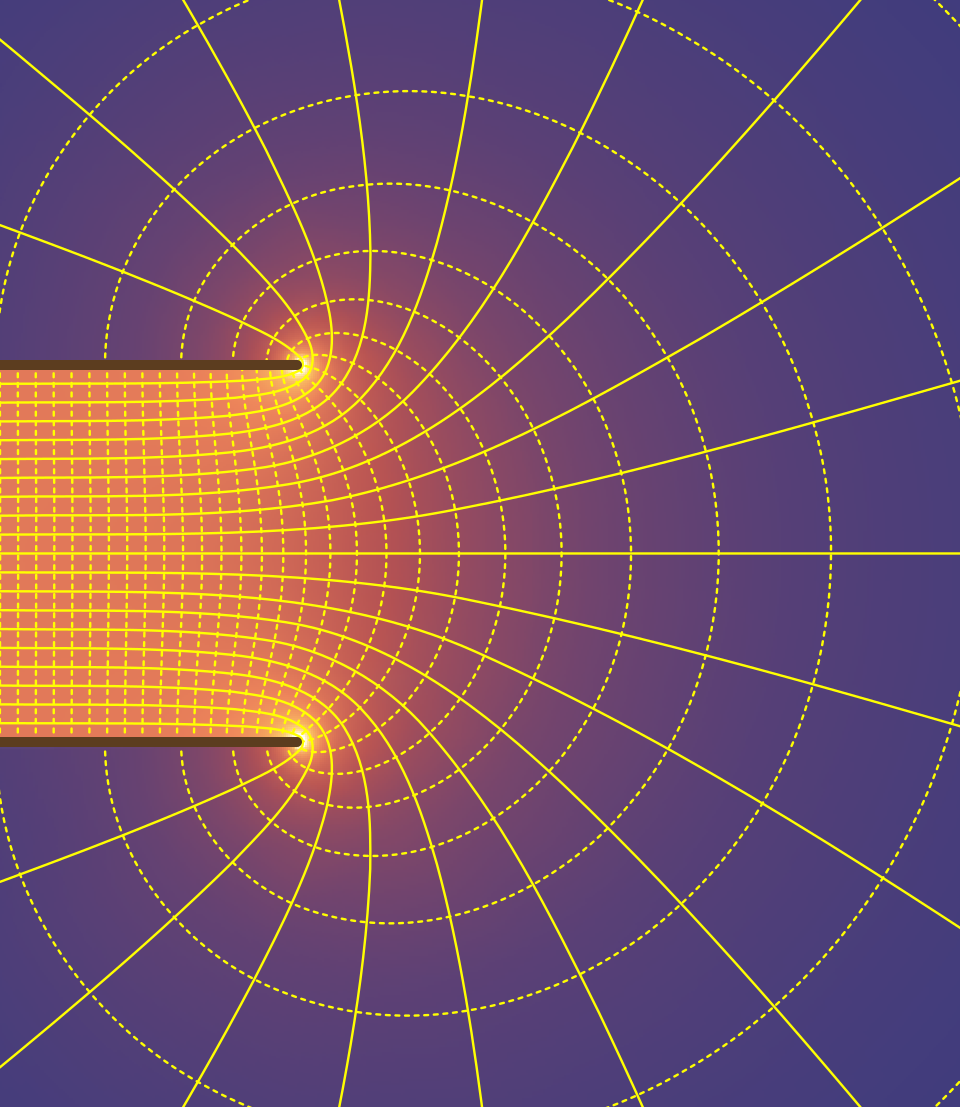
\includegraphics[width=0.6\textwidth]{parallel-plate-capacitor}}
\end{figure}
\begin{figure}[!ht]
    \ffigbox[\FBwidth]{%
        \caption{Example of a figure with a caption spanning just the width of the figure.}%
        \label{fig:tighter_caption}%
    }{\includegraphics[width=0.6\textwidth]{example-image-a}}
\end{figure}

\clearpage
\begin{example}[Multi-Paragraph Figure Caption with Verbatim Text]
    It is possible to have multi-paragraph captions for figures.
    One must remember to provide a short description as \macro{\caption[This is a Short Description]{...}}, or else \LaTeX{} will complain.

    See \Cref{fig:multi-paragraph_verbatim_figure} for an example, demonstrating also a workaround for typesetting verbatim text in contexts where \enquote{fragile} commands are not allowed.
\end{example}
\begin{figure}[!ht]
    \includegraphics[width=0.6\textwidth]{example-image-b}
    \caption[Necessary to provide short description.]{
        Example of a figure with a multi-paragraph caption.

        Notice the spacing between the paragraphs.
        It was customized using the \fakemacro{parskip} key in \fakemacro{\captionsetup} provided by the \package{caption} package.

        To typeset verbatim text in the caption, use the \fakemacro{\fakeverb{...}} command instead of the usual \fakemacro{\verb|...|}, which is not allowed in captions.
    }%
    \label{fig:multi-paragraph_verbatim_figure}%
\end{figure}

\section{Appendix Section}%
\label{sec:Appendix Section}

Note the numbering of various environments in the appendix.

\begin{definition}[Math in the Description --- \(\sin(\alpha)\approx\alpha\)]
    This is an example definition in an Appendix.
    Note the automatic switch to the alternative sans math font in the Definition description.
\end{definition}

\begin{remark}
    The page header reflects that this is an appendix page.
\end{remark}


\backmatter
\references

\end{document}
